\documentclass[a4paper]{article}
\usepackage[utf8]{inputenc}
\usepackage[T1]{fontenc}
\usepackage[spanish]{babel}
\usepackage{a4wide}
\usepackage{amsmath}
\usepackage{amssymb,amsfonts,textcomp}
\usepackage{color}
\usepackage{array}
\usepackage{supertabular}
\usepackage{hhline}
\usepackage{hyperref}
\usepackage{fancyhdr}
\usepackage[table]{xcolor}
%\hypersetup{pdftex, colorlinks=true, linkcolor=blue, citecolor=blue, filecolor=blue, urlcolor=blue, pdftitle=, pdfauthor=, pdfsubject=, pdfkeywords=}
\usepackage[pdftex]{graphicx}
% footnotes configuration
\makeatletter
\renewcommand\thefootnote{\arabic{footnote}}
\makeatother
% Text styles
\newcommand\textstyleStrongEmphasis[1]{\textbf{#1}}
% Outline numbering
\setcounter{secnumdepth}{0}
\makeatletter
\newcommand\arraybslash{\let\\\@arraycr}
\makeatother
% List styles
\newcommand\liststyleWWNumxxix{%
\renewcommand\labelitemi{{}-}
\renewcommand\labelitemii{o}
\renewcommand\labelitemiii{[F0A7?]}
\renewcommand\labelitemiv{[F0B7?]}
}
\newcommand\liststyleLi{%
\renewcommand\labelitemi{{\textbullet}}
\renewcommand\labelitemii{${\circ}$}%
\renewcommand\labelitemiii{${\blacksquare}$}
\renewcommand\labelitemiv{{\textbullet}}
}
\newcommand\liststyleLii{%
\renewcommand\labelitemi{{\textbullet}}
\renewcommand\labelitemii{${\circ}$}
\renewcommand\labelitemiii{${\blacksquare}$}
\renewcommand\labelitemiv{{\textbullet}}
}
\newcommand\liststyleLiii{%
\renewcommand\labelitemi{{\textbullet}}
\renewcommand\labelitemii{${\circ}$}
\renewcommand\labelitemiii{${\blacksquare}$}
\renewcommand\labelitemiv{{\textbullet}}
}
\newcommand\liststyleLiv{%
\renewcommand\labelitemi{{\textbullet}}
\renewcommand\labelitemii{${\circ}$}
\renewcommand\labelitemiii{${\blacksquare}$}
\renewcommand\labelitemiv{{\textbullet}}
}
\newcommand\liststyleLv{%
\renewcommand\labelitemi{{\textbullet}}
\renewcommand\labelitemii{${\circ}$}
\renewcommand\labelitemiii{${\blacksquare}$}
\renewcommand\labelitemiv{{\textbullet}}
}
\newcommand\liststyleLvi{%
\renewcommand\labelitemi{{\textbullet}}
\renewcommand\labelitemii{${\circ}$}
\renewcommand\labelitemiii{${\blacksquare}$}
\renewcommand\labelitemiv{{\textbullet}}
}
\newcommand\liststyleLvii{%
\renewcommand\labelitemi{{\textbullet}}
\renewcommand\labelitemii{{\textbullet}}
\renewcommand\labelitemiii{{\textbullet}}
\renewcommand\labelitemiv{{\textbullet}}
}
\newcommand\liststyleLviii{%
\renewcommand\labelitemi{{\textbullet}}
\renewcommand\labelitemii{{\textbullet}}
\renewcommand\labelitemiii{{\textbullet}}
\renewcommand\labelitemiv{{\textbullet}}
}
\newcommand\liststyleLix{%
\renewcommand\labelitemi{{\textbullet}}
\renewcommand\labelitemii{{\textbullet}}
\renewcommand\labelitemiii{{\textbullet}}
\renewcommand\labelitemiv{{\textbullet}}
}
\newcommand\liststyleLx{%
\renewcommand\labelitemi{{\textbullet}}
\renewcommand\labelitemii{{\textbullet}}
\renewcommand\labelitemiii{{\textbullet}}
\renewcommand\labelitemiv{{\textbullet}}
}
% Page layout (geometry)
\setlength\voffset{-1in}
\setlength\hoffset{-1in}
\setlength\topmargin{2cm}
\setlength\oddsidemargin{2cm}
\setlength\textheight{24.203001cm}
\setlength\textwidth{17.001cm}
\setlength\footskip{0.0cm}
\setlength\headheight{0.998cm}
\setlength\headsep{0.499cm}
% Footnote rule
\setlength{\skip\footins}{0.119cm}
\renewcommand\footnoterule{\vspace*{-0.018cm}\setlength\leftskip{0pt}\setlength\rightskip{0pt plus 1fil}\noindent\textcolor{black}{\rule{0.25\columnwidth}{0.018cm}}\vspace*{0.101cm}}
% Pages styles
\makeatletter
\newcommand\ps@Standard{
  \renewcommand\@oddhead{[Warning: Draw object ignored]}
  \renewcommand\@evenhead{\@oddhead}
  \renewcommand\@oddfoot{}
  \renewcommand\@evenfoot{}
  \renewcommand\thepage{\arabic{page}}
}
\newcommand\ps@FirstPage{
  \renewcommand\@oddhead{}
  \renewcommand\@evenhead{}
  \renewcommand\@oddfoot{}
  \renewcommand\@evenfoot{}
  \renewcommand\thepage{\arabic{page}}
}
\makeatother

\setlength\tabcolsep{1mm}
\renewcommand\arraystretch{1.3}
\title{}
\author{}
\date{2013-06-03}

\renewcommand{\baselinestretch}{1.2}

\begin{document}

\pagestyle{empty}
\setcounter{page}{0}


\includegraphics[width=3cm]{logo-uclm.jpg}
\hfill

\includegraphics[width=3cm]{logo-esii.png}

{\centering \par}
\begin{center}

\includegraphics[width=2.96cm,height=3.522cm]{logo-conciti.png}
\end{center}

\vskip 3em
{\centering\bfseries\large
UNIVERSIDAD DE CASTILLA-LA MANCHA
\par}

\vskip 3em
{\centering\bfseries\large
ESCUELA SUPERIOR DE INFORMÁTICA
\par}

{\centering\bfseries\large
Departamento de Sistemas Informáticos\footnote{DEPARTAMENTO DE SISTEMAS INFORMÁTICOS o DEPARTAMENTO DE
INGENIERÍA ELÉCTRICA, ELECTRÓNICA, AUTOMÁTICA Y COMUNICACIONES o DEPARTAMENTO DE MATEMÁTICAS o cualquier otro
de la UCLM al que pertenezca el director. \par }
\par}

\vskip 3em
{\centering\bfseries\large
ANTEPROYECTO DEL TRABAJO FIN DE GRADO
\par}

{\centering\bfseries\large
GRADO EN INGENIERÍA INFORMÁTICA
\par}

{\centering\bfseries\large
TECNOLOGÍA ESPECÍFICA DE / INTENSIFICACIÓN / ITINERARIO DE \footnote{INGENIER\'IA DEL SOFTWARE o INGENIER\'IA DE COMPUTADORES o COMPUTACI\'ON o
TECNOLOG\'IAS DE LA INFORMACI\'ON (esta \'ultima est\'a tambi\'en asociada a los TFG del \textbf{curso} de
\textbf{adaptaci\'on})}
\par}

\vskip 3em
{\centering\bfseries
(Título del TFG)
\par}

\vfill % Rellena espacio automáticamente hasta ajustar al margen inferior 

Autor: Fernando Luján Martínez

Director: Gregorio Díaz Descalzo
\footnote{Sólo en el caso de que haya un segundo director.} (nombre y apellidos)

\vskip 1em 
\mbox{\begin{minipage}[b][2.5cm][c]{0.7\linewidth} {\large Mes, 2018}  \end{minipage}}
\hfill % Rellena espacio automáticamente hasta que la image se ajuste a la derecha
\mbox{
\includegraphics[width=2.5cm]{logo-euroinf.png}}
\vskip 1em %Un línea en blanco para que el logo de Euroinf no se pegue al footnote

\clearpage\pagestyle{empty}
\thispagestyle{FirstPage}

\setcounter{tocdepth}{10}
\renewcommand\contentsname{\'Indice de contenido}
\tableofcontents

\clearpage
\pagestyle{empty}

El anteproyecto recoger\'a, en un \textcolor[rgb]{0.5019608,0.0,0.0}{m\'aximo de 10 p\'aginas}, los siguientes
apartados:

\liststyleWWNumxxix
\begin{itemize}
\item Introducci\'on (muy recomendable aunque no obligatorio)
\item Tecnolog\'ia espec\'ifica cursada por el alumno
\item Objetivos
\item M\'etodo y fases de trabajo
\item Medios que se pretenden utilizar
\item Bibliograf\'ia b\'asica consultada en la elaboraci\'on del anteproyecto
\item Contrato de propiedad intelectual (si lo hubiera)
\end{itemize}

\section{1.\ INTRODUCCI\'ON}

El cap\'itulo de introducci\'on podr\'a abordar los siguientes aspectos:

\liststyleWWNumxxix
\begin{itemize}
\item Introducci\'on al tema, entorno en el que el trabajo desempe\~nar\'a su objetivo, \ justificaci\'on de la
importancia del trabajo abordado.
\item Motivaci\'on y antecedentes (con algunas referencias bibliogr\'aficas).
\item Descripci\'on gr\'afica del proyecto (es aconsejable incorporar una figura que describa el trabajo a desarrollar y
que mejore la comprensi\'on del mismo).
\end{itemize}

En la actualidad vivimos inmersos en un mundo de información, cualquier sistema por simple que que sea genera una gran cantidad de datos. Poder analizar todo lo que se genera para obtener información relevante es uno de los objetivos que se persiguen. Esto se puede hacer de diferentes formas, la primera que podemos imaginarnos es guardar y después analizar. De esta premisa nace el concepto de big data. Este procedimiento tiene una serie de ventajas y desventajas, se necesita (mucho) espacio de  almacenamiento, lo que guardemos puede no ser tan valioso como se pensaba o que los resultados del análisis no son inmediatos y hasta que no tengamos suficientes datos no podemos llegar a ninguna conclusión.

Para evitar las desventajas comentadas, principalmente la tercera donde en según que sectores es imprescindible tener conocimiento al instante del estado en el que se encuentran. La siguiente opción entonces es analizar en tiempo real los datos que se van generando, de esta forma no es necesario el almacenamiento de datos y los resultados de los análisis están conforme se generan/reciben los datos, listos para la toma de decisiones.

Este segundo procedimiento también es muy útil en entornos complicados en lo que no es posible tener un extenso almacenamiento, la conexión para la transferencia de datos no tiene un gran ancho de banda, la velocidad o la fiabilidad en la entrega de todos los paquetes no es la mejor.

En el caso en que nos centraremos (poner aquí que sera de placas solares) esta claro que todo lo indicado arriba se cumple:

\begin{itemize}
\item normalmente las plantas fotovoltaicas están ubicadas lejos de núcleos urbanos grandes, por esto la conexión hacia el exterior no es idónea.
\item Poner un sistema que almacene y examine los datos tampoco es interesante en términos de mantenimiento y por tanto económicos.
\item Aunque la extensión de una de estas plantas es variable suelen ser de al menos unas hectáreas. Por tanto si estamos tratando de detectar fallos en alguno de los componentes, ir componente por componente sería inviable.
\item Por último, incluso obviando lo anterior y siendo capaces de almacenar y analizar los datos si algo esta dañado cuando interesa saberlo es lo antes posible y no una semana después, todo esto sin perder el potencial de detectarlos aunque sean complejos.
\end{itemize}

Por estas razones el procesamiento complejo de eventos (CEP o de sus siglas en inglés Complex Event Processing) es perfecto para ser aplicado en el entorno indicado porque... (desarrollo de que es cep)

En este Trabajo Fin de Grado lo que trataremos es de la mano de Ingeteam desarrollar un sistema capaz de detectar eventos y lo que es más interesante patrones de eventos. Estos nos serán indicados por sus técnicos.

\begin{figure}[h]
    \centering
    {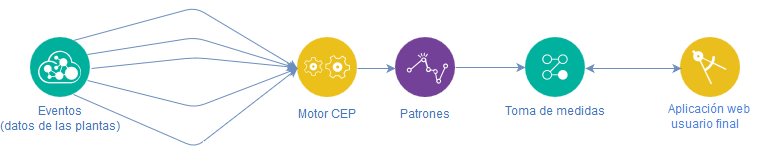
\includegraphics[width=\textwidth]{vision_general_fase_3.png}}
    \caption{esquema general para comprender mejor el objetivo que persigue el proyecto.}
    \label{fig:mesh1}
\end{figure}

En líneas generales, tendremos una serie de datos que llegarán de los campos solares, estos datos los llamaremos eventos porque son considerados sucesos que incluyen una marca de tiempo. Toda esta información se filtrará y acondicionara para el motor CEP donde estarán incluidos los patrones de eventos que desarrollaremos. Cuando el motor detecte a partir de los eventos que ha recibido un patrón se tomaran una serie de medidas, como puede ser el envío de una alerta a un técnico. Esto lo podemos ver graficamente en la figura \ref{fig:mesh1}.

\section{2. TECNOLOG\'IA ESPEC\'IFICA / INTENSIFICACIÓN / ITINERARIO CURSADO POR EL ALUMNO}
El Trabajo Fin de Grado (TFG, de ahora en adelante) siempre deber\'a demostrar la aplicaci\'on de las competencias
generales de la titulaci\'on. Adem\'as, el TFG deber\'a aplicar \textbf{algunas} de las competencias espec\'ificas
asociadas a la \textbf{Tecnolog\'ia Espec\'ifica o Intensificaci\'on} que el alumno ha cursado. Por lo tanto, el alumno
incluir\'a en el anteproyecto \textbf{dos tablas}. Una tabla para seleccionar la tecnolog\'ia cursada y en la que se
contextualiza el TFG:


\bigskip

{\centering\bfseries
Tabla 1. Tecnolog\'ia Espec\'ifica cursada por el alumno
\par}

\begin{center}
\tablefirsthead{}
\tablehead{}
\tabletail{}
\tablelasttail{}
\begin{supertabular}{m{6.803cm}}
 \rowcolor{gray!50}
{\bfseries Marcar la Tecnolog\'ia Cursada}
\\\hline
~

Tecnolog\'ias de la Informaci\'on\\
\rowcolor{gray!30}
~

Computaci\'on\\
~

Ingenier\'ia del Software \hfill x\\
\rowcolor{gray!30}
~

Ingenier\'ia de Computadores\\\hline
\end{supertabular}
\end{center}



\clearpage\pagestyle{plain}
\thispagestyle{FirstPage}

\ \ En la segunda tabla, el alumno deber\'a justificar c\'omo \textbf{algunas} de las competencias espec\'ificas de la
intensificaci\'on se aplicar\'an o tomar\'an forma en el TFG, \textbf{La relaci\'on de competencias por
intensificaci\'on se encuentran en el Anexo I al final de este documento. }


\bigskip
{\centering\bfseries
Tabla 2. Justificaci\'on de las competencias espec\'ificas abordadas en el TFG
\par}
\begin{center}
	%\newcolumntype{C}{>{\centering} m{1cm} }
  \begin{supertabular}{m{5.605cm}m{10.849cm}}
  	\iffalse
    	primera fila, cabecera
    \fi
    \rowcolor{gray!50}
	{\color{black} \textbf{Competencias}} &
	{\color{black} \textbf{Justificaci\'on}}\\\hline
    
    {\color{black} Competencia 1} &
    {\color{black} La justificación de esta competencia la desmigaré en tres partes.
    {\begin{itemize} 
    \item primero la metodología de desarrollo que utilizaré será scrum junto con prototipado.
    \item Segundo, las tecnologías utilizadas serán el lenguaje Esper EPL y su un motor cep. [cuando hagamos la reunión esto lo terminaré para ver como encajo lo del poi del principio y como se mostraran los resultados del final]
    \item --como hago el mantenimiento, porque no voy a mantenerlo--
    \item Para evaluar el proyecto desde el principio se aplicaran pruebas unitarias y pruebas de integración
    \end{itemize}}
    }\\
    
    \rowcolor{gray!30}
    {\color{black} Competencia 2} &
    {\color{black} Para la toma de requisitos al cliente y más adelante todo case se harán reuniones periódicas al principio y al final de cada iteración.
    La elicitación de los requisitos se hará con historias de usuario. Esto es así porque del resto de posibilidades que nos quedan, como pueden ser los casos de uso, no son lo más adecuado a la metodología que vamos a utilizar.\newline
    Por otro lado para dejar claro que lo realizado en las iteraciones se ajusta a lo definido inicialmente cada historia de usuario tendrá una prueba de aceptación, relativa al prototipo que se entregue.}\\
    
    {\color{black} Competencia 3} &
    {\color{black} --para hacer esta sección tengo que hacer la reunión con los de ingeteam para saber como vamos a meter lo que desarrolle en su entorno real}\\
    
    \rowcolor{gray!30}
    {\color{black} Competencia 4} &
    {\color{black} Poner ¿Por qué es bueno cep para este problema?
    El problema que vamos a tacar es detectar ciertos desgastes y futuros fallos en todo el sistema que hay detrás de una o varias plantas fotovoltaicas. Para ello vamos a analizar todos los datos generados de las placas de estos campos. Al ser una gran cantidad, el monitóreo de las instalaciones debe de ser en tiempo real, los resultados del análisis de los datos deben de estar lo antes posible y por último inferir, a priori, inferir los datos para obtener esos resultados no es una tarea trivial, por tanto podemos decir que la opción que mejor se ajusta a estos requisitos es cep}\\
    
    {\color{black} Competencia 5} &
    {\color{black} algunos motores cep: 
      \begin{itemize}
        \item \href{https://flink.apache.org/index.html}{flint}
        \item \href{https://docs.jboss.org/drools/release/6.2.0.CR3/drools-docs/html/DroolsComplexEventProcessingChapter.html}{drools}
        \item \href{https://github.com/wso2/siddhi
    y https://wso2.com/products/complex-event-processor/}{Siddhi} and \href{https://wso2.com/products/complex-event-processor/}{WSO2}
        \item \href{https://cloud.google.com/solutions/architecture/complex-event-processing}{Google Cloud Platform}
        \item \href{http://www.oracle.com/technetwork/middleware/complex-event-processing/documentation/index.html}{Real Time Streaming Analytics Oracle}
        \item \href{http://www.espertech.com/esper/}{Esper}
      \end{itemize}
      Poner otras metodologías mas y porque hemos optado por scrum junto con prototipado
      -- cuando sepa después de las reunión otras tecnologías que vaya a utilizar las miraré
   	}\\
    
    \rowcolor{gray!30}
    {\color{black} Competencia 6} &
    {\color{black} desarrollar que lo vamos a hacer en tes fases/springs y porque es bueno hacerlo así y posibles riesgos potenciales de esta planificación}\\

\end{supertabular}
\end{center}
\bigskip

\section{3. \ OBJETIVOS}
De acuerdo a la Introducci\'on, el alumno deber\'a especificar cu\'al o cuáles son las hip\'otesis de trabajo de las
que se parten, qu\'e se pretende resolver, y en base a eso formular el objetivo principal del TFG.

El objetivo principal deber\'a desglosarse en sub-objetivos parciales. Los sub-objetivos deberán describirse de forma breve y concisa.

Como pre\'ambulo a la formulaci\'on del objetivo parcial, el alumno deber\'a discutir sobre las limitaciones y
condicionantes a tener en cuenta en el desarrollo del TFG (lenguaje de desarrollo, equipos, madurez de la tecnolog\'ia,
etc.).

Del mismo modo, ser\'a recomendable incluir una lista preliminar de requisitos del sistema a construir.

\section[4. M\'ETODO Y FASES DE TRABAJO]{4. M\'ETODO Y FASES DE TRABAJO}

\bigskip

Para el desarrollo del proyecto, el alumno deber\'a seguir alg\'un proceso o metodolog\'ia af\'in al problema que
pretende resolver. Para ello, deber\'a aportar una peque\~na descripci\'on del proceso o metodolog\'ia (no m\'as de una
p\'agina) y \textbf{justificar su adecuaci\'on al problema a resolver}.

Del mismo modo, el alumno podrá realizar una breve planificaci\'on de la ejecuci\'on del proyecto seg\'un el proceso
o metodolog\'ia seleccionada.

Como parte de la descripci\'on del m\'etodo y las fases de trabajo, el alumno podr\'a incluir una descripci\'on
preliminar de las tareas, una planificaci\'on temporal, diagramas de Gantt o recursos similares que pueda considerar
necesarios.

Si hubiera m\'as de una metodolog\'ia que a juicio del alumno podr\'ia ser af\'in al proyecto, \'estas deber\'an
mencionarse, y justificar la que considera m\'as adecuada (esto puede considerarse parte de la justificaci\'on a la
adecuaci\'on al problema a resolver).

\section{5. MEDIOS QUE SE PRETENDEN UTILIZAR}
\section{5.1. Medios Hardware}

El alumno deber\'a describir los medios hardware que prev\'e ser\'an necesarios para el desarrollo del proyecto.

\section{5.2. Medios Software}

El alumno deber\'a describir los medios software (lenguajes, entornos de desarrollo, herramientas de gesti\'on y
planificaci\'on, etc.) que prev\'e ser\'an necesarios para el desarrollo del proyecto

%\clearpage\pagestyle{empty}
%\thispagestyle{FirstPage}

\section[6. REFERENCIAS]{6. REFERENCIAS}
En esta secci\'on se incluir\'an todas las referencias bibliogr\'aficas, ordenadas alfab\'eticamente por el primer
apellido del primer autor, de las obras de las cuales se haya realizado alguna cita en los apartados anteriores. Las
referencias deber\'an contener datos b\'asicos como nombre y apellidos de los autores, t\'itulo de la obra, evento al
que pertenece, p\'aginas, fecha y lugar de celebraci\'on (si se tratara de art\'iculos de congreso), ISBN, editorial y
ciudad (si se tratara de libro), nombre de revista, p\'aginas, volumen y n\'umero (si se tratara de revista), etc.

Se emplear\'a un formato de referencia reconocido en el \'ambito acad\'emico como
ACM\footnote{http://www.acm.org/sigs/publications/proceedings-templates}\footnote{http://www.cs.ucy.ac.cy/\~{}chryssis/specs/ACM-refguide.pdf}.
Otros formatos aconsejables son, por ejemplo, IEEE, AMA, APA y AMA.

Ejemplos de referencias con formato ACM:

\liststyleLi
\begin{itemize}
\item Para un art\'iculo de revista:
\end{itemize}
Bowman, M., Debray, S. K., and Peterson, L. L. 1993. Reasoning about naming systems. \textit{ACM Trans. Program. Lang.
Syst.} 15, 5 (Nov. 1993), 795-825. DOI= \url{http://doi.acm.org/10.1145/161468.16147}.

\liststyleLii
\begin{itemize}
\item Para un informe t\'ecnico
\end{itemize}
Ding, W. and Marchionini, G. 1997. \textit{A Study on Video Browsing Strategies. Technical Report}. University of
Maryland at College Park.

\liststyleLiii
\begin{itemize}
\item Para un libro

Tavel, P. 2007. \textit{Modeling and Simulation Design.} AK Peters Ltd., Natick, MA, USA.
\end{itemize}
\liststyleLiv
\begin{itemize}
\item Para un cap\'itulo de libro:
\end{itemize}
Greiner, R. 1999. Explanation-based learning. In Wilson and F. Keil, R. eds. \textit{The Encyclopedia of Cognitive
Science}, MIT Press, Cambridge, MA, USA. 301-303.

\liststyleLv
\begin{itemize}
\item Para un art\'iculo en las actas de un congreso:
\end{itemize}
Fr\"ohlich, B. and Plate, J. 2000. The cubic mouse: a new device for three-dimensional input. In \textit{Proceedings of
the SIGCHI Conference on Human Factors in Computing Systems} (The Hague, The Netherlands, April 01 - 06, 2000). CHI
'00. ACM, New York, NY, 526-531. DOI= \url{http://doi.acm.org/10.1145/332040.332491}.

\liststyleLvi
\begin{itemize}
\item Para un p\'agina de Internet (con autores conocidos)

Steele, B. Look, Ma, no wires! Cornell class project tests wireless networking, \textit{Cornell Chronicle, 31 }(35).
Retrieved February 15, 2004, from Columbia University:
\url{http://www.news.cornell.edu/Chronicle/00/5.18.00/wireless_class.html}
\item Para un p\'agina de Internet (con autores desconocidos)

MIT Project Oxygen: Overview, 2004. Retrieved March 15, 2005, from Computer Science and Artificial Intelligence
Laboratory, Massachusetts Institute of Technology: \url{http://oxygen.lcs.mit.edu/Overview.html}. \
\end{itemize}

\bigskip

\section{7. CONTRATO DE PROPIEDAD INTELECTUAL (si lo hubiera)}

\bigskip

\clearpage\clearpage\pagestyle{plain}
\thispagestyle{FirstPage}


\bigskip
\end{document}
